
\section{linear PCA: Recap}

\begin{frame}\frametitle{\secname}
\begin{itemize}
\item Requires \pause

 centering the data.
\only<2>{
\slidesonly{
\begin{center}
	
\includegraphics[width=0.2\textwidth]{img/mem_notthisagain}%
\end{center}
}
}

\pause
 
\item Eigenvalue problem: $\vec C\,\vec e = \lambda \vec e$
\item limited to \underline{linear} correlations
\end{itemize}


\begin{center}
	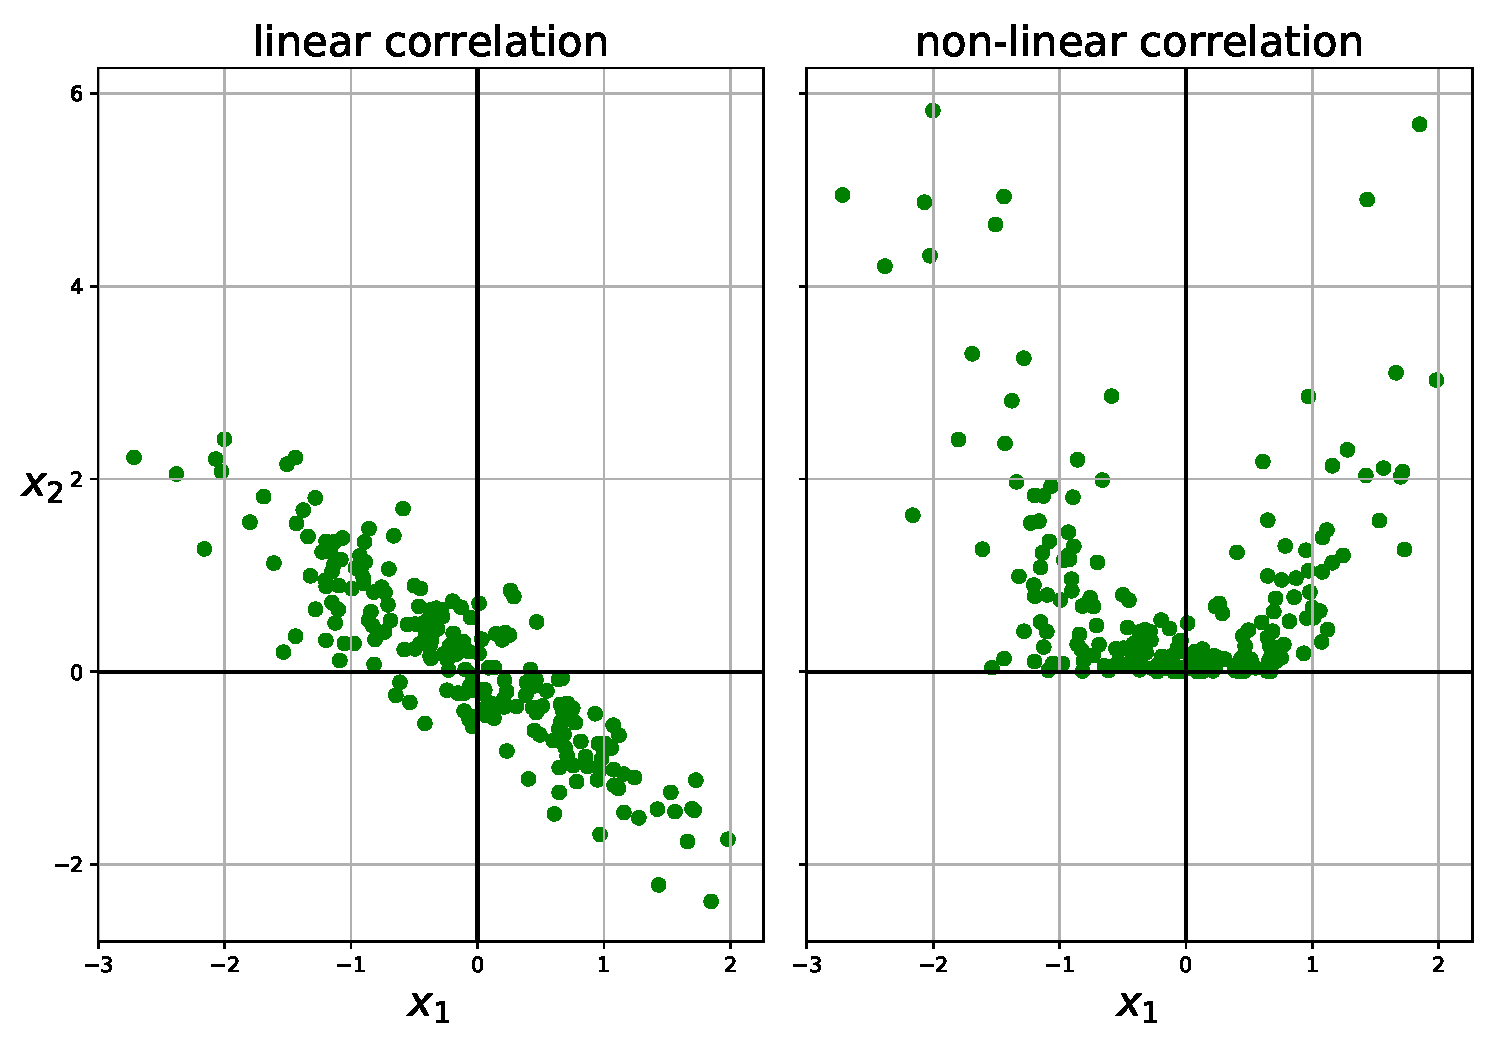
\includegraphics[width=0.5\textwidth]{img/scatter}%
	\captionof{figure}{linear vs. non-linear correlations}
\end{center}

Kernel PCA for finding non-linear features.\\


\end{frame}

\begin{frame}\frametitle{What is Kernel PCA about?}

Don't panic! Kernel PCA is essentially standard linear PCA applied to a non-linearly transformed version of the data.

\begin{center}
	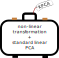
\includegraphics[width=0.3\textwidth]{img/koffer}%
\end{center}

\end{frame}
